\documentclass[compress]{beamer}
\usepackage[utf8]{inputenc}
\usepackage{hyperref}

\usepackage{tikz}
\usetikzlibrary{graphs, quotes, arrows.meta, matrix}

\usetheme{default}
\usecolortheme{Nord}
\setbeamertemplate{navigation symbols}{}

\title{Segment Tree}
\subtitle{Problemi}
\author{Lorenzo Ferrari, Davide Bartoli}
\date{\today}

\begin{document}

\begin{frame}
    \maketitle
\end{frame}

\begin{frame}{Table of contents}
  \tableofcontents
\end{frame}

\section{Segment Tree}
\begin{frame}{Segment Tree}{Idea}
    Per rispondere efficientemente a query\footnote{siano esse somma, minimo, o operazioni pi\`u complesse} su un range $[l, r]$ di valori, ci salviamo la risposta per alcuni intervalli la cui lunghezza \`e una potenza di $2$.
    \vfill
    \makebox[\textwidth]{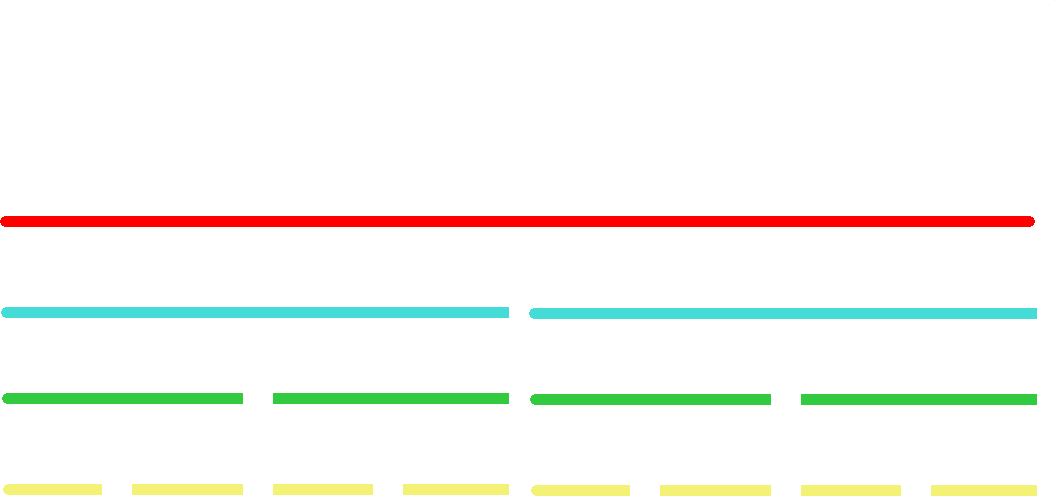
\includegraphics[scale=.70]{./img/intervalli.png}}
    \vfill
    \pause
    Gli intervalli sono in totale $N + N/2 + N/4 + \dots \leq 2N$
\end{frame}

\begin{frame}{Segment Tree}{Idea}
    L'insieme di intervalli si pu\`o vedere come un albero binario, che rende pi\`u intuitiva l'implementazione.\\ 
    \vfill
    \makebox[\textwidth]{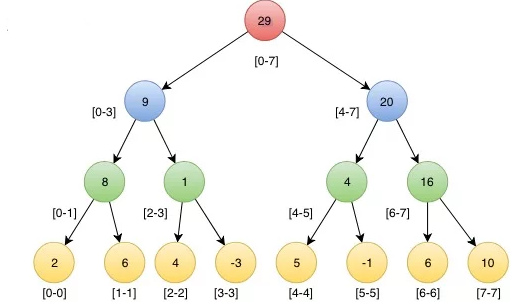
\includegraphics[scale=.50]{./img/segment_tree.png}}
\end{frame}

\begin{frame}{Segment Tree}{caratteristiche}
    Nominiamo i nodi a partire da $1$ per livelli: la radice ha indice $1$, il secondo livello contiene i nodi $2$ e $3$, il terzo livello i nodi $4$, $5$, $6$ e $7$ \dots\\
    \pause
    L'albero binario cos\`i costruito ha le seguenti caratteristiche:
    \begin{itemize}
        \item la radice ha indice $1$
        \item il figlio sinistro di un nodo $i$ ha indice $2i$
        \item il figlio destro di un nodo $i$ ha indice $2i + 1$
        \item il padre di un nodo $i$ ha indice $i/2$
        \item i nodi sono numerati da $1$ a $2N - 1$
        \item l'albero ha altezza $O(\log N)$
    \end{itemize}
\end{frame}

\begin{frame}
    \makebox[\textwidth]{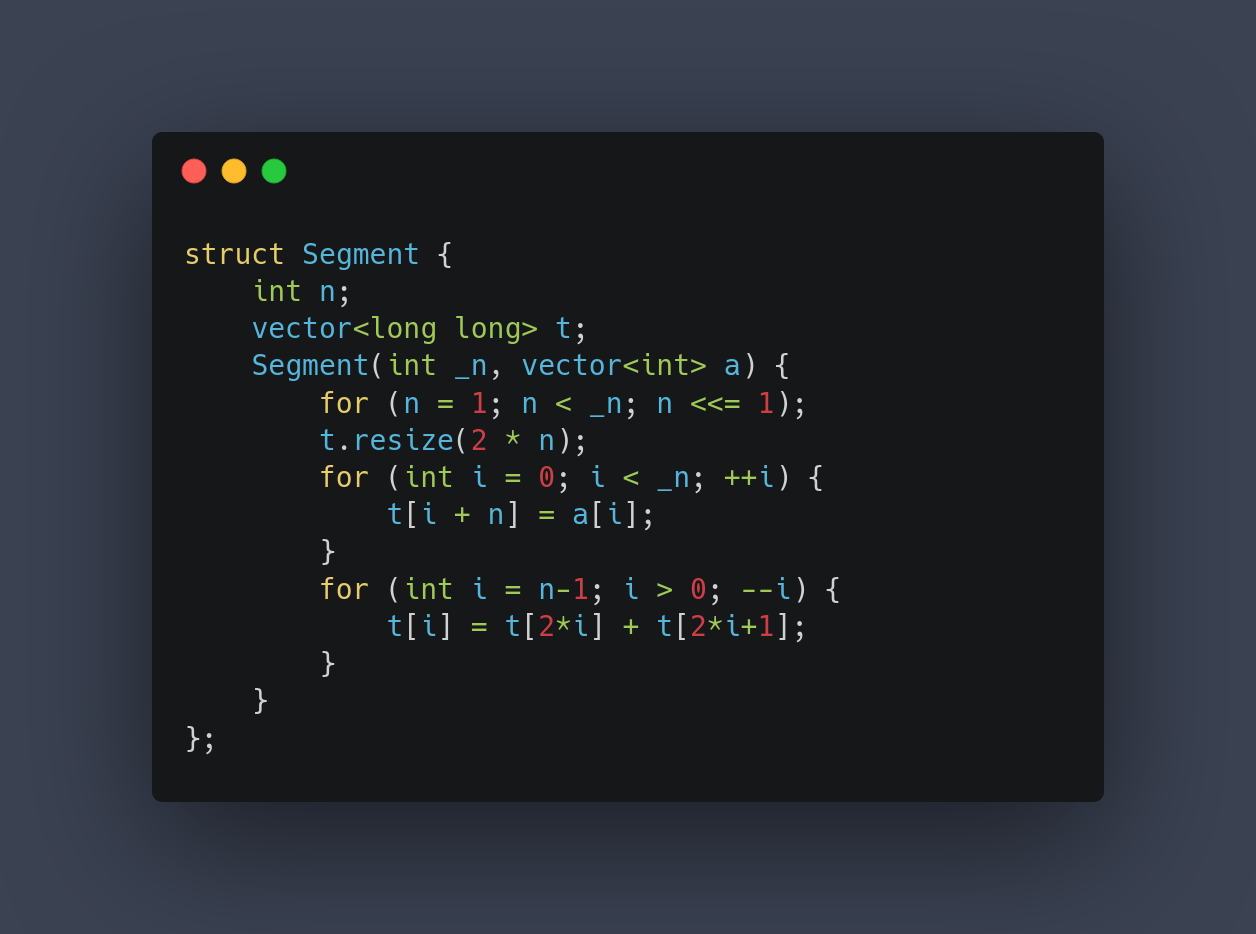
\includegraphics[scale=.3]{./img/st_build.png}}
\end{frame}

\begin{frame}{Segment Tree}{Update}
    Per gli \textbf{update}, notiamo che ogni nodo è contenuto in esattamente $\log N $ intervalli, possiamo quindi aggiornarli tutti in $O(\log N)$.
\end{frame}

\begin{frame}
    \makebox[\textwidth]{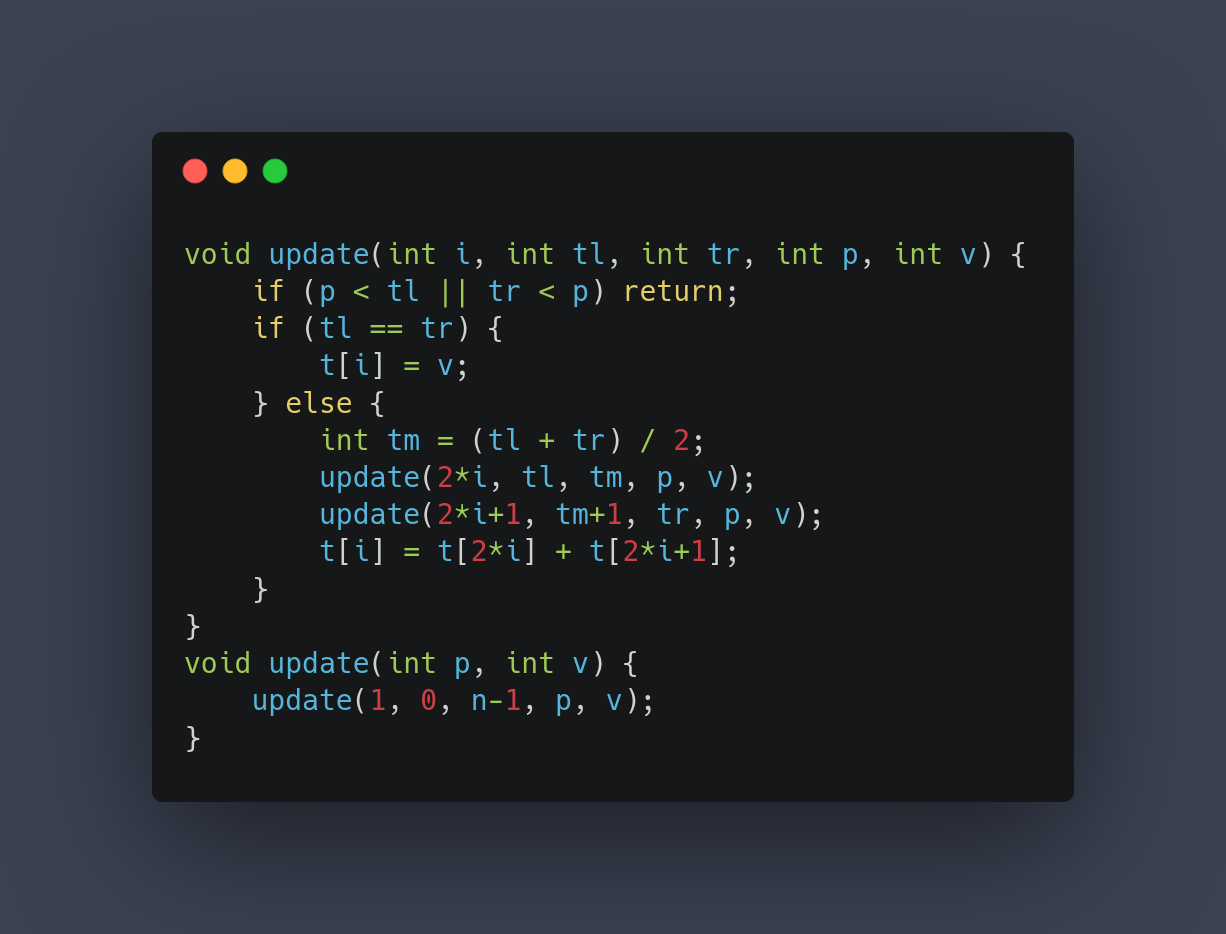
\includegraphics[scale=.3]{./img/st_update_rec.png}}
\end{frame}

\begin{frame}
    \makebox[\textwidth]{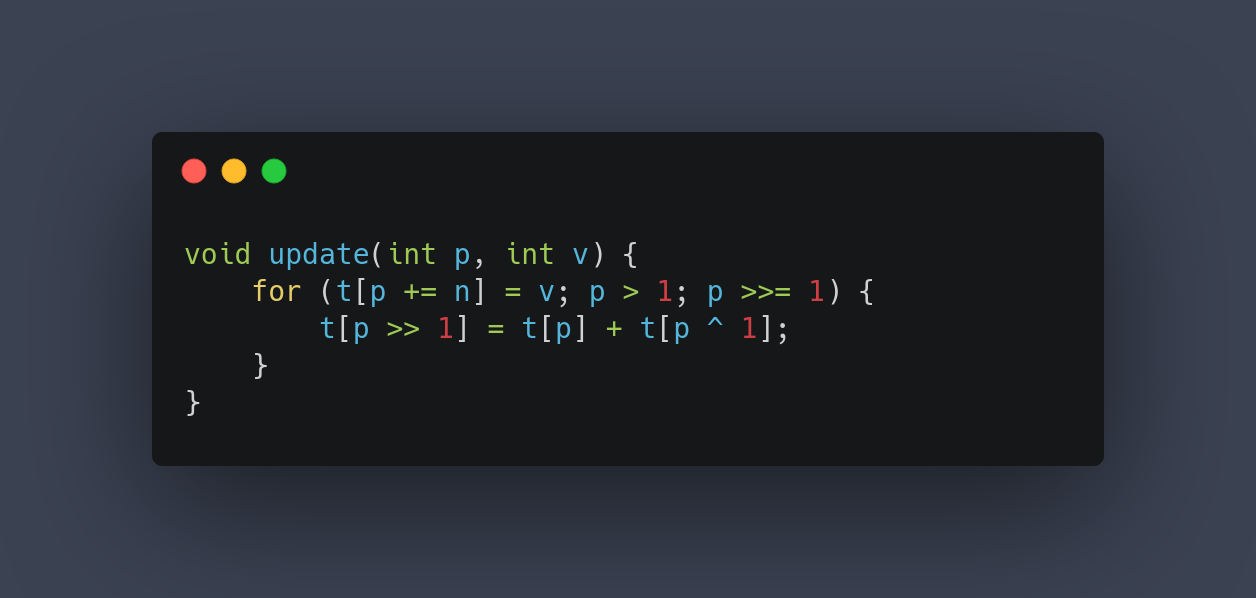
\includegraphics[scale=.3]{./img/st_update.png}}
\end{frame}

\begin{frame}{Segment Tree}{Query}
    Per le \textbf{query} dobbiamo trovare un insieme di intervalli da unire per ottenere la risposta desiderata.\\
    \vfill
    \makebox[\textwidth]{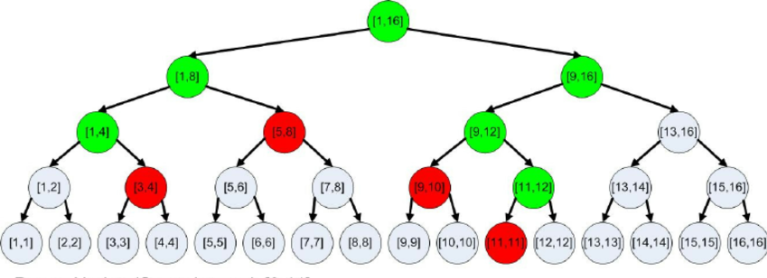
\includegraphics[scale=.40]{./img/query.png}}
\end{frame}

\begin{frame}{Segment Tree}{Query}
    Per rispondere a una generica query $[l, r]$, possiamo utilizzare una dfs sull'albero. Ogni volta che raggiungiamo un nodo abbiamo $3$ possibilit\`a:\\
    \pause
    \begin{itemize}
        \item l'intervallo \`e completamente contenuto in $[l, r]$, quindi possiamo aggiungerlo alla risposta e fermarci
        \item l'intervallo \`e completamente fuori da $[l, r]$, quindi possiamo ignorarlo e fermarci
        \item l'intervallo \`e parzialmente contenuto in $[l, r]$, quindi ricorriamo nei figli
    \end{itemize}
    \pause
    Si pu\`o dimostrare che questo processo visita $O(\log N)$ nodi.
    \vfill
    \pause
    Questa struttura dati impiega solo $O(\log N)$ per query/update.
\end{frame}

\begin{frame}
    \makebox[\textwidth]{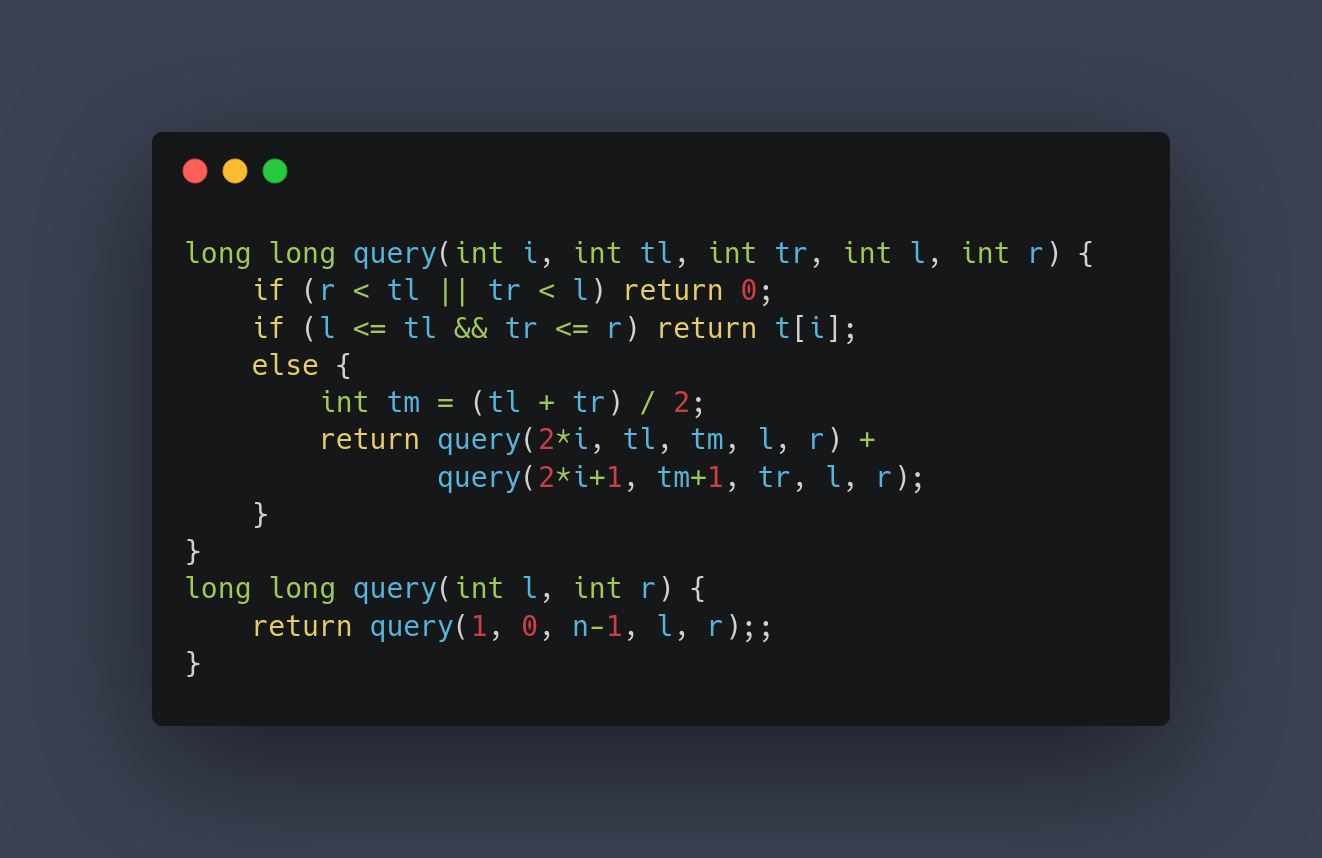
\includegraphics[scale=.3]{./img/st_query.png}}
\end{frame}

\begin{frame}
    Il segment nell'implementazione fa update e calcola la somma su range in $O(\log N)$, ma i segment tree sono strutture dati molto generiche e versatili, che si possono utilizzare per risolvere molti altri problemi.\\
    \pause
    \vfill
    \begin{block}{In generale $\dots$}
    Se si salvano le informazioni su un intervallo in una \texttt{struct nodo} e le informazioni del padre si possono facilmente ottenere combinando le informazioni dei figli, allora si pu\`o usare un segment tree.
    \end{block}
    \vfill
\end{frame}

\section{Maximum Subarray Sum}
\begin{frame}{Maximum Subarray Sum}{Problema}
    \begin{exampleblock}{Maximum Subarray Sum}
        Dato un array di $N$ numeri, rispondi alle seguenti query:
        \begin{itemize}
            \item modifica il valore di un elemento
            \item calcola la somma massima di un sottoarray di un intervallo $[l, r]$
        \end{itemize}
    \end{exampleblock}
    \underline{\url{https://training.olinfo.it/\#/task/rangetree3/statement}}
    \pause
    Cerchiamo di capire come utilizzare un segment tree per risolvere questo problema.
\end{frame}

\begin{frame}{Maximum Subarray Sum}{idea}
    Come avevamo visto la scorsa volta, per poter utilizzare il segment tree è necessario riuscire a unire le informazioni di 2 nodi velocemente.\\
    \pause
    Quali informazioni dobbiamo salvarci per risolvere questo problema? Come facciamo a unire le informazioni di 2 nodi?\\
    \pause
    Sicuramente una delle informazioni è la somma massima di un sottoarray, ovvero quello che ci chiede il problema.\\
    \pause
    Come facciamo a unire 2 nodi per\'o?\\
\end{frame}

\begin{frame}{Maximum Subarray Sum}{idea}
    \makebox[\textwidth]{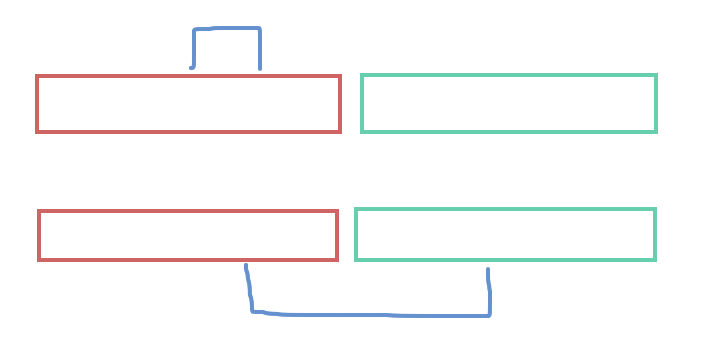
\includegraphics[scale=.3]{./img/max_subarray.png}}
    \vfill
    Ci sono 2 casi:
    \begin{itemize}
        \item l'intervallo massimo è completamente contenuto in uno dei 2 nodi, quindi conosciamo gi\'a il suo valore
        \item l'intervallo è a met\`a tra i 2 nodi
    \end{itemize}
    \pause
    Nel secondo caso non abbiamo modo di calcolare il valore che ci interessa: dobbiamo tenerci altre informazioni nei nodi.\\
\end{frame}

\begin{frame}{Maximum Subarray Sum}{idea}
    Notiamo che in questo caso il subarray massimo è formato da un suffisso del primo nodo e un prefisso del secondo nodo.\\
    \pause
    Possiamo salvarci quindi anche il prefisso e il suffisso massimi di ogni nodo.\\
    \pause
    Riusciamo però a unire 2 nodi e calcolare il suffisso massimo e il prefisso massimo del nodo padre? Al momento no.
\end{frame}

\begin{frame}{Maximum Subarray Sum}{idea}
    Consideriamo solo il prefisso per ora.
    \vfill
    \makebox[\textwidth]{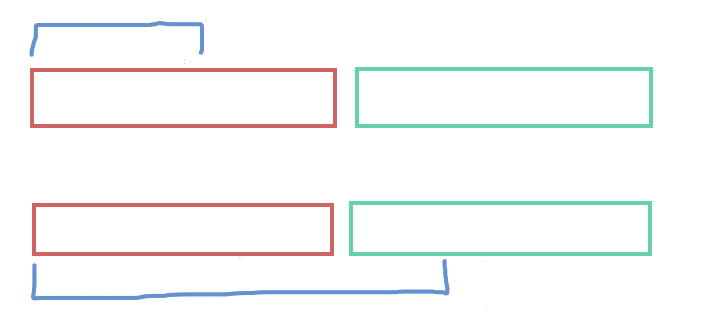
\includegraphics[scale=.3]{./img/prefisso_massimo.png}}
    \vfill
    \pause
    Anche in questo caso abbiamo 2 casi, e notiamo che ci basta salvare la somma totale del nodo per avere finalmente tutte le informazioni necessarie.
\end{frame}

\begin{frame}{Maximum Subarray Sum}{implementazione}
    \vfill
    \makebox[\textwidth]{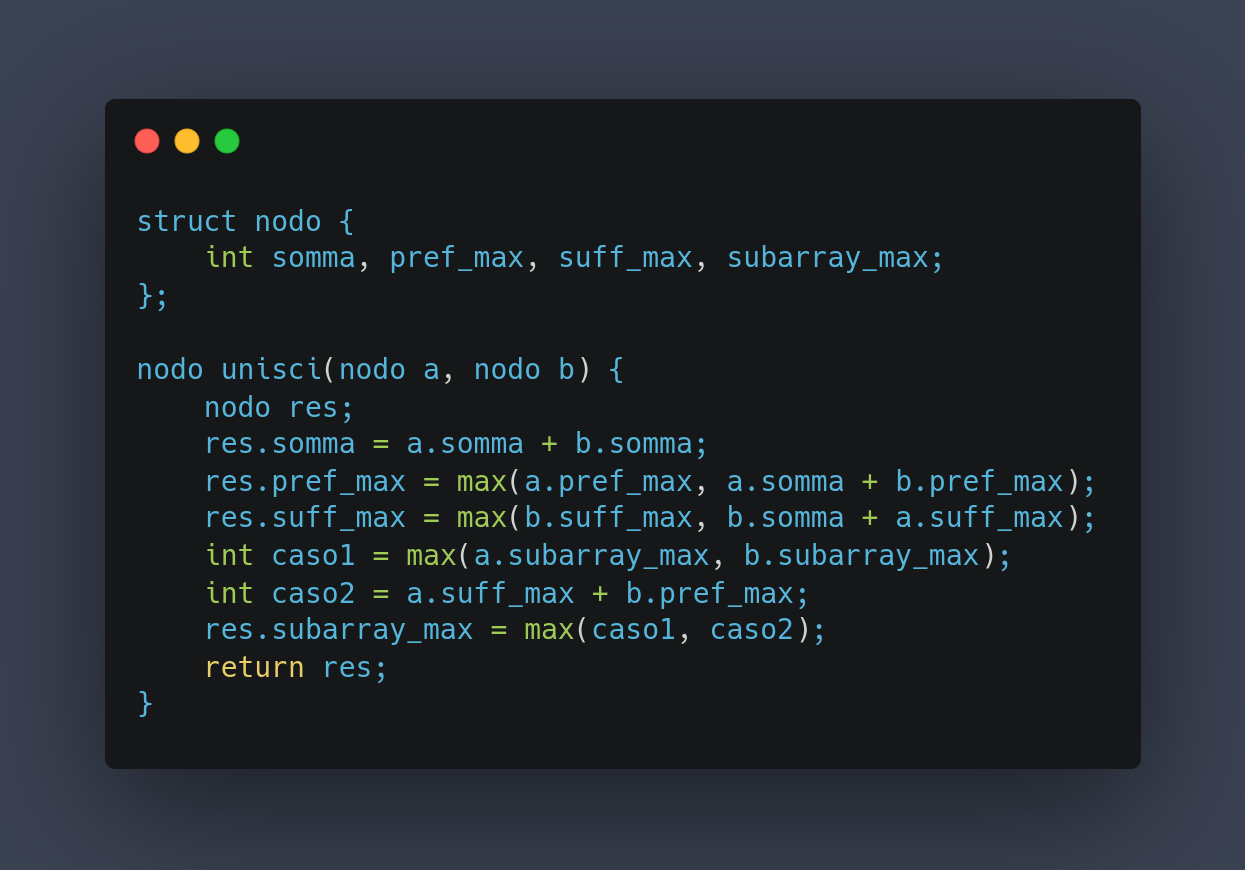
\includegraphics[scale=.26]{./img/max_sub_impl.png}}
    \vfill
\end{frame}

\begin{frame}{Conta elementi}{Problema}
    \begin{exampleblock}{Conta elementi}
        Dato un array di $N$ numeri, rispondi alla seguente query:
        \begin{itemize}
            \item quanti sono gli elementi $\ge k$ nell' intervallo $[l, r]$
        \end{itemize}
    \end{exampleblock}
    \pause
    In questo problema non abbiamo update, ma un segment tree può comunque farci molto comodo per risolvere il problema.\\
    \pause
    In particolare se sappiamo calcolare la risposta per un nodo velocemente, calcolare la risposta in $[l, r]$ è semplice: ci basta 
    sommare le risposte dei nodi che formano $[l, r]$.
\end{frame}

\begin{frame}{Conta elementi}{idea}
    Come facciamo a calcolare la risposta per un nodo?\\
    \pause
    Possiamo salvare in ogni nodo una lista ordinata dei valori che contengono, e calcolare la risposta facendo una ricerca binaria.\\
    \pause
    Questo è possibile dato che non dobbiamo fare update, quindi una volta inizializzato il segment tree non viene più modificato.\\
    \pause
    Ma quanta memoria stiamo usando in questo caso? Avevamo visto che ogni nodo è compreso in esattamente $\log N$ intervalli, 
    quindi la memoria totale è $O(N \log N)$, e non abbiamo problemi.
\end{frame}

\section{lower\_bound query}
\begin{frame}{lower\_bound query}
    Alcune query possono chiedere di trovare il primo (o l'ultimo) elemento $\geq x$ in un range $[l, r]$.
    \pause
    \vfill
    Un'opzione \`e fare una binary search con $\log (r-l)$ query di minimo, per un costo totale di $O(\log^2 n)$
    \pause
    \vfill
    Il problema pu\`o per\`o essere risolto in $O(\log n)$. Come succede spesso con i segment tree, risolviamo il problema ricorsivamente e tronchiamo la ricerca quando nell'intervallo in cui siamo non ci sono soluzioni (l'elemento massimo \`e $< x$).
    \vfill
\end{frame}

\section{Problemi}

\begin{frame}{Problemi}
    \small{\underline{\url{https://cses.fi/problemset/task/1650}}}
    \small{\underline{\url{https://cses.fi/problemset/task/2206}}}
    \small{\underline{\url{https://training.olinfo.it/\#/task/muraglia/statement}}}
    \small{\underline{\url{https://training.olinfo.it/\#/task/rangetree3/statement}}}
    \small{\underline{\url{https://training.olinfo.it/\#/task/ois_panama/statement}}}
    \small{\underline{\url{https://training.olinfo.it/\#/task/pre-egoi-parkour/statement}}}
\end{frame}

\end{document}
